\section{Task and Method}
\label{sec:framework}
\label{sec:framework:problem}

The input is a list of triples $G$, source text $X$, a fixed document ID
$h_0$, and allowed relations $\mathcal R_X$. The list can contain copies
of the same triple. Each relation has at most one nonempty value.
Examples include document fields and receipt fields.
The scorer uses the reference graph $G^*$ to check the output.

The main method has three steps: clean the input, ask a model for a complete
graph, and filter the triples. The prompt can include an error report or
source-line hints. The filter checks each value against the source text.
Reference scores and human review measure output quality.

Figures~\ref{fig:framework_overview} and~\ref{fig:optimization_flow} show a
second path. A learned router gives weights to edits. A selector tries the
edits on graph copies and chooses one at a time.
Section~\ref{sec:impl:optimizer_audit} tests this path with saved proposals.

\begin{figure}[t]
    \centering
    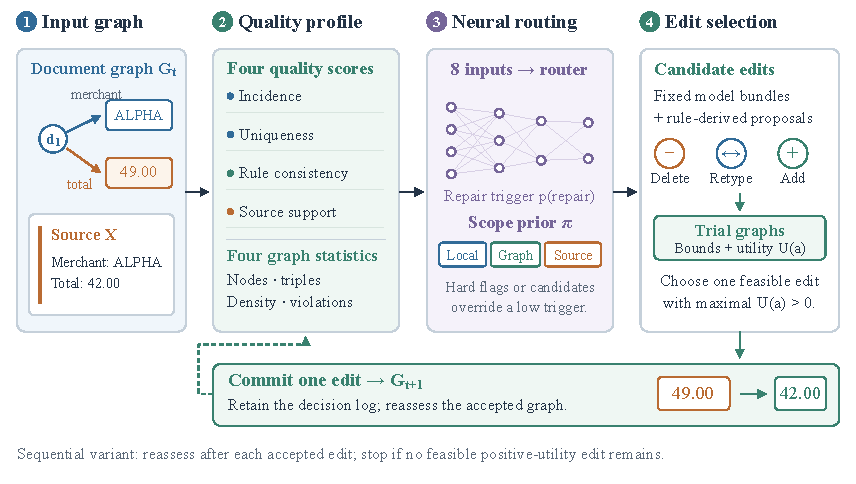
\includegraphics[width=0.98\textwidth]{figure/method/image1.pdf}
    \caption{Repair by choosing edits one at a time. Four quality scores and four
graph counts feed the learned router. It gives a repair score and weights
for three kinds of edits. The selector tries model and rule edits on graph
copies. It applies the allowed edit with the highest positive score, then
checks the graph again. Section~\ref{sec:impl:optimizer_audit} gives this test.}
    \label{fig:framework_overview}
\end{figure}

\subsection{Input Cleanup and Error Report}
\label{sec:framework:profile}

Figure~\ref{fig:scale_relationship} groups the checks into local, graph,
and source checks. They count copies, check the document ID and relation,
and look for the value in the text.

\begin{figure}[t]
    \centering
    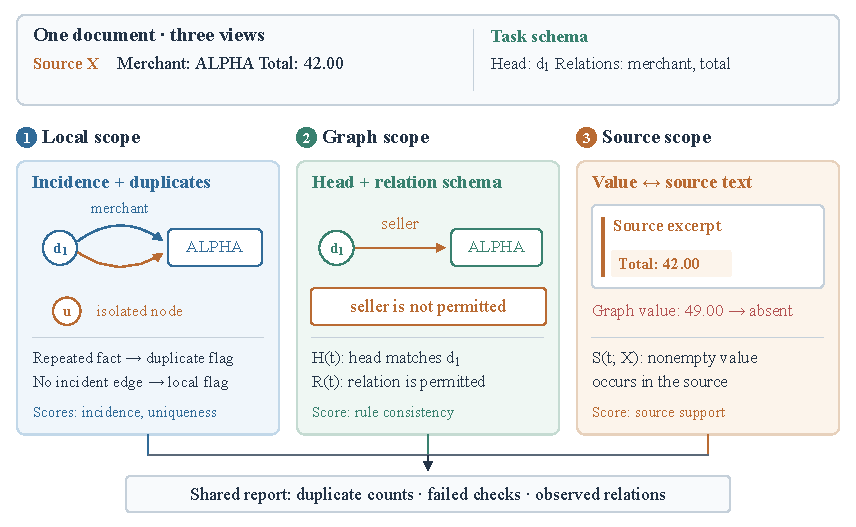
\includegraphics[width=0.98\textwidth]{figure/method/image2.pdf}
    \caption{Three groups of graph checks: repeated facts and unlinked nodes
(local), invalid relations (graph), and values missing from the text
(source). Both repair paths use these groups. Their report follows
Eq.~(\ref{eq:diagnostic_predicates}).}
    \label{fig:scale_relationship}
\end{figure}

The preprocessor $P$ removes duplicate triples. It reverses an edge if its
object is $h_0$ and its subject is a different node. It then removes triples
with an invalid head or relation. Here, the head is the subject of a triple.
The cleaned graph is $G_s=P(G;h_0,\mathcal R_X)$.

For a triple $t=(h,r,o)$, the three checks are
\begin{equation}
    \label{eq:diagnostic_predicates}
    H(t)=\mathbf1[h=h_0],\quad
    R(t)=\mathbf1[r\in\mathcal R_X],\quad
    S(t;X)=\mathbf1[o\ne\emptyset\ \wedge\ o\text{ occurs in }X].
\end{equation}
$H$ checks the document ID, $R$ checks the relation, and $S$ checks whether
the nonempty value occurs in the text.
The error report stores duplicate counts, failed-check positions,
and relations in $G_s$:
\begin{equation}
    \label{eq:diagnostic_context}
    D(G_s,X)=\big(n_{\mathrm{dup}},I_H,I_R,I_S,\mathcal R(G_s)\big).
\end{equation}
For example, $I_S=\{i:S(t_i;X)=0\}$ lists positions that fail the source
check. The report uses the cleaned input. Cleanup removes some errors
before the report is built. We test the effect of adding this report to the
prompt. Fields are optional, and the main method calls the model once for
every document to recover missing values.

\subsection{Generating a Graph from Source Text}
\label{sec:framework:architecture}

The language model returns an ordered list of triples:
\begin{equation}
    \label{eq:proposal_generation}
    C=L_\theta(X,h_0,\mathcal R_X,G_s,D(G_s,X)).
\end{equation}
The prompt asks for a complete graph. It tells the model to copy values from
the text, keep correct fields, and fill missing or wrong values.
The JSON parser returns an empty graph for an invalid response.
Scoring includes these empty graphs. The base prompt uses the same source,
input graph, model settings, and output limit, with the error report removed.

\subsection{Checking the Generated Triples}
\label{sec:framework:constraints}

The gate is a filter. It keeps triples that pass
Eq.~(\ref{eq:diagnostic_predicates}) and keeps at most one value per relation.
Let $\operatorname{uniq}(C)$ remove copies in output order. The triples that
pass the checks are
\begin{equation}
    \label{eq:eligible_candidates}
    C_X=\{t\in\operatorname{uniq}(C):H(t)R(t)S(t;X)=1\}.
\end{equation}
The allowed output sets are
\begin{equation}
    \label{eq:admissible_subsets}
    \mathcal F(C_X)=\left\{A\subseteq C_X:
    \sum_{t\in A}\mathbf1[r_t=r]\leq1,\ \forall r\in\mathcal R_X\right\}.
\end{equation}
The filter scans the triples in order. For each relation, it keeps the first
triple that passes the checks. The output $\widehat G$ has size
\begin{equation}
    \label{eq:selection_size}
    |\widehat G|=\max_{A\in\mathcal F(C_X)}|A|
    =|\{r:\exists t\in C_X,\ r_t=r\}|.
\end{equation}
Each relation forms one group with room for one triple.
The filter keeps one triple from each group that has a valid candidate.
It thus keeps the largest allowed number of candidates.
The first valid value in output order wins when several values pass.

\subsection{Field Meanings and Source Lines}
\label{sec:framework:field_evidence}

A receipt can list a brand name, a company name, a subtotal, and a final
amount. We give each field a short meaning to help the model choose its
value. All receipt repair methods receive these meanings and numbered
source lines.

The source-line index adds hints for each field. Fixed patterns find company
terms, address terms, postcodes, dates, and total labels. Each matching line
is an anchor. The index includes that line, one line before it, and two
lines after it. Simple receives the full source and field meanings.
Evidence Index also receives the line hints.

The receipt filter uses the same whitespace rule as the parser.
$N(s)$ changes each run of spaces or line breaks to one space and trims the
ends. The source check is
\begin{equation}
    S_{\mathrm{ws}}(t;X)=\mathbf1[|N(o)|>0\ \wedge\
    N(o)\text{ occurs in }N(X)].
\end{equation}
It keeps word boundaries, case, and punctuation. The receipt follow-up uses
this check. Earlier tests use the original exact-text check.
\section{Implementation}
\label{sec:implementation}

\subsection{Repair Steps}
\label{sec:impl:assessment}

Algorithm~\ref{alg:abstract} gives Diagnosis + Gate.
Diagnosis is the error report. Gate is the triple filter.
Code builds the report and runs the checks. The model proposes field values.

\begin{algorithm}[t]
\caption{Repair with source text and field checks}
\label{alg:abstract}
\begin{algorithmic}[1]
\Require Input triples $G$, source $X$, document ID $h_0$, allowed relations $\mathcal R_X$
\Ensure Repaired graph $\widehat G$ and rejection log $J$
\State $G_s\gets P(G;h_0,\mathcal R_X)$
\State $D\gets D(G_s,X)$
\State $C\gets\textsc{Parse}(L_\theta(X,h_0,\mathcal R_X,G_s,D))$
\State $\widehat G\gets\emptyset$; $J\gets\emptyset$; $B\gets\emptyset$
\For{each candidate $t=(h,r,o)$ in generation order}
    \If{$t$ appeared earlier in $C$}
        \State append $(t,\text{duplicate})$ to $J$
    \ElsIf{$H(t)R(t)S(t;X)=1$ and $r\notin B$}
        \State $\widehat G\gets\widehat G\cup\{t\}$; $B\gets B\cup\{r\}$
    \Else
        \State append $(t,\text{failed check})$ to $J$
    \EndIf
\EndFor
\State \Return $\widehat G,J$
\end{algorithmic}
\end{algorithm}

The runner passes the source, document ID, allowed relations, and input
triples to the model. The scorer loads the reference values.
Tests change reference values and defect labels and check that model inputs
stay the same. The older data loader reads the document ID from the
reference record as task information.

With hash-based lookups, cleanup takes $O(|G|)$ triple operations on average.
Filtering $k$ candidates costs $O(k(1+c_X))$ and uses
$O(k+|\mathcal R_X|)$ extra memory. Here, $c_X$ is the cost of finding a
value in the text. Text length affects this cost. We time model calls
apart from these checks.

\subsection{Comparing Prompt Context and Filtering}
\label{sec:impl:enhancement}

One system prompt supports three settings: basic input, input with an error
report, and input with SHACL checks. Three calls give three responses for
each input. We score each response before and after filtering, giving six
scores. Each before/after pair uses the same triples.

The model is \texttt{google/gemma-4-26B-A4B-it} at temperature zero.
The output limit is 4,000 tokens in each setting. We report input tokens
because the prompt lengths differ. Request times include retries and pacing
waits. We save all responses and include invalid responses in scoring.
The earlier Claude tests compare methods with their own prompts.

\subsection{SHACL Prompt Baseline}
\label{sec:impl:shacl}

Lin et al.\ use five prompt parts: an introduction, detected errors,
SHACL rules, graph context, and instructions \citep{ref_lin2025}.
We use their full-rules/full-graph ($M+G$) setting for the field task.
The pySHACL tool checks document IDs, allowed relations, nonempty values,
and field counts. A SPARQL rule checks values against the source text.

The prompt includes the full source and returns a complete JSON graph.
It groups each document's errors into one call. We call this baseline
\emph{Lin-style SHACL context (adapted)}. RDF stores unique triples.
Our shared JSON input keeps duplicate copies. We score the output before
and after filtering for each prompt setting.

\subsection{Choosing Edits One at a Time}
\label{sec:impl:optimizer_audit}

\begin{figure}[t]
    \centering
    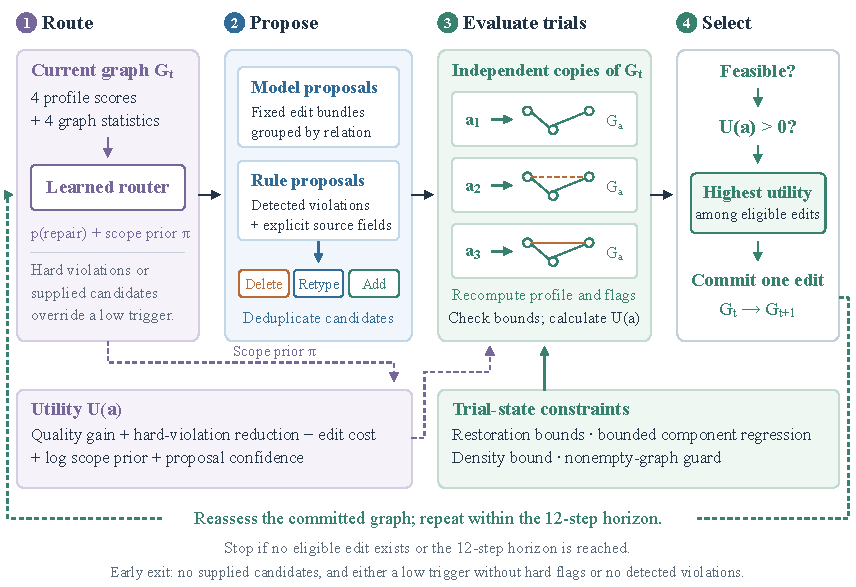
\includegraphics[width=0.98\textwidth]{figure/method/image3.pdf}
    \caption{One step of edit selection. The router gives a repair score and
edit-type weights. Each model or rule edit is tried on a graph copy.
Graph bounds decide which edits are allowed. The selector applies the edit
with the highest positive score, saves the decision, and checks again.
The test allows up to twelve steps.}
    \label{fig:optimization_flow}
\end{figure}

Figure~\ref{fig:optimization_flow} gives the edit-selection steps in
Figure~\ref{fig:framework_overview}. The profile has four scores:
the share of nodes linked by edges ($Q_{\mathrm{inc}}$), triple uniqueness
($Q_{\mathrm{uniq}}$), rule agreement ($Q_{\mathrm{rule}}$), and source
support ($Q_{\mathrm{src}}$). The router receives these scores $\mathbf{s}$
and four graph counts $\mathbf{g}$: nodes, triples, density, and violations.
It returns repair probability $p_{\mathrm{repair}}$ and edit-type weights
$\boldsymbol{\pi}$. These weights form the scope prior. The selector uses
them with quality gains, edit costs, and graph bounds to score trial edits.

A rule error or supplied candidate starts the trial checks even when
$p_{\mathrm{repair}}<\tau_{\mathrm{repair}}$. If both are absent, the selector
stops. It applies the allowed edit with the highest positive score.
It keeps the graph and stops if all edit scores are zero or negative.
After each edit, it computes the profile and router outputs again.

For this test, we group changes between the cleaned input and model output
by relation. Each group is one edit bundle. Candidate confidence is 0.7.
The run allows 12 steps. Each trial graph must meet the graph bounds.
We compare learned weights with an always-on uniform prior, which gives
equal weight to each edit type. Both use the default score settings.

Logs save every trial graph, profile, score, decision, and stop reason.
Source matching removes whitespace from the source and value.
The archive also stores the earlier logs that used different whitespace
rules for the two strings. Algorithm~\ref{alg:abstract} and the edit selector
have separate tests.

% Begin merged sections/math_revision.tex
\subsection{Shared Features for Training and Use}
\label{sec:impl:profile_revision}

Training and repair use the same eight input features: four quality scores,
node count, triple count, density, and detected-violation count.
The density uses distinct directed node pairs. Training labels describe
the added defects. The model weights and feature scaler store a feature
version. A version mismatch switches the router to equal weights.
The document ID and allowed relations are task inputs.

The source-field check finds values after allowed field labels at the
start of a document, line, or sentence. It reports a missing field when
the text gives a value and the graph omits it. The check skips a field if
repeated labels give conflicting values. These reports enter the violation
count and candidate list. The node-link score counts connected nodes.
A partial star graph can have a node-link score of 100.

Hierarchy checks use the direction of management, supervision, and membership
relations. They skip relations with unclear meanings. Entity checks apply
to endpoints marked as entity references. Other field values are treated
as text. Each edit or bundle passes the empty-graph check.
A supplied candidate receives a trial check even if the repair probability
is low or the graph has no detected violation.

Let $Q\in[0,100]$ be profile quality, $h$ the rule-error count, $c(a)$
the edit cost, $s(a)$ its type, and $z(a)$ its confidence.
The default edit score is
\begin{equation}
\begin{split}
U(a)={}&\frac{Q(G_a)-Q(G)}{100}
+0.20\frac{\max(0,h(G)-h(G_a))}{\max(1,h(G))}\\
&-0.35c(a)+0.05\log\!\left(\max(\pi_{s(a)},0.05)+10^{-6}\right)
+0.02z(a).
\end{split}
\end{equation}
Here, $G_a$ is the trial graph. Delete, retype, and add costs are 0.30,
0.16, and 0.06. A bundle's cost is the sum of its edit costs.
The selector applies the allowed edit with the highest positive score.
The four quality scores have equal weights.
Trial graphs keep all bounds already met. A score below its lower bound
must stay the same or increase. A checked score can fall by at most two
points, subject to these bounds. Trials also meet the density bound.
Comparing pairs of triples costs $O(m^2)$ for $m$ triples.
$T$ rounds with up to $K$ trials per round cost $O(TKm^2)$, plus text checks.
The main filter scans the candidate list once.

A second score subtracts $0.05\log(1/3+10^{-6})$ from the default score.
This sets the prior term to zero for equal weights. It keeps the edit order
for a fixed router but shifts the point at which scores become positive.
Both scores are fixed before the saved-proposal tests.
% End merged sections/math_revision.tex
